% chap4.tex
%

\mychapter{Non-factoid Question Answering}
\label{chapter:non-factoid}

\noindent

In this chapter I summarize the proposed work in developing a non-factoid question answering system.
In particular, Section \ref{sec:non-factoid:architecture} described the general architecture of the system, and the following chapters describe the proposed improvements to different stages of the pipeline.

\section{The architecture of the system}
\label{sec:non-factoid:architecture}

\begin{figure}[h]
\centering
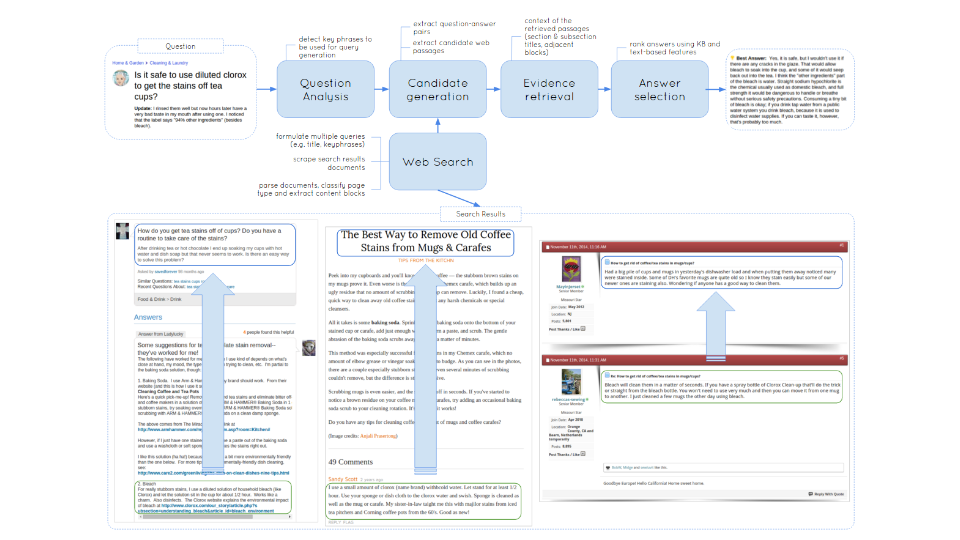
\includegraphics[width=\textwidth]{img/web_page_structure_nonfactoid}
\caption{Using web page structure information for non-factoid question answering}
\label{fig:non-factoid:architecture}
\end{figure}

The architecture of the system I develop is somewhat standard and contains 4 main stages: question analysis, candidate generation, evidence retrieval and answer selection.
Figure \ref{fig:non-factoid:architecture} depicts the question-answering pipeline.

\subsection{Question Analysis}
\label{sec:non-factoid:architecture:analysis}

Questions that users post to CQA websites often contain title and body and can be relatively long and contain multiple important and not so important context information and details.
The success of the retrieval-based question answering system depends on the information it finds in a collection.
Extra long search queries are not very efficient and can return few or zero results.
Therefore, there is a problem of summarizing the user question.
Some strategies often used include considering first part of the question, \eg title of the question only.
However, often the most important part of the question isn't the title, or the title doesn't contain all the crucial information, \eg\\
\textbf{Title}: \textit{Diet please please help asap?}\\
\textbf{Body}: \textit{I want to lose weight, at least 4 stone but I don't know what I should eat :( what should I have for breakfast lunch and dinner? Should I exercise a little? Please help!!}

To summarize the question I propose to use recent advances in the field of deep learning, in particular a model similar to \cite{rush-chopra-weston:2015:EMNLP}.
In more detail, I propose to train neural network based summarization model to generate the summary of the question, which will be used as a query to retrieve similar questions.
Such a model can be specifically trained to maximize retrieval performance on a collection of question-answer pairs, retrieved by systems in LiveQA TREC 2015 and labeled by NIST assessors.

\subsection{Structure of the Web Page for Candidate Generation and Scoring}
\label{sec:non-factoid:architecture:page-structure}

The diversity and complexity of non-factoid questions pose additional challenges for automatic question answering systems.
To answer such questions a system often needs to provide a whole paragraph of text, \eg TREC LiveQA'15 limits the answers to a maximum of 1000 characters.
Therefore, a candidate answer becomes much longer, which requires additional attention on candidate generation and ranking stages.

% Is this related work? Or here?
Existing techniques usually extract one or more consecutive sentences not exceeding the maximum answer length, pool them together and rank using certain feature representation, by large ignoring the context information from the page where the answer was extracted from.
In the system I develop I propose to utilize the structure of the web page for both candidate generation and scoring.

To generate better candidates I'm going to utilize the structure of retrieved web pages.
The previous analysis showed \cite{savenkov_liveqa15}, that many search results retrieved for the question are FAQs, forums or other community question answering websites.
From such resources it's beneficial to extract question answer pairs, which can be done either be designing wrapper for popular websites, utilizing semantic annotations, such as \hyperref[https://schema.org]{https://schema.org} or by applying some of the automatic question-answer extraction methods \cite{cong2008finding}.
For other resources, page segmentation techniques, similar to \cite{cai2003vips}, can split a page into semantically information blocks, which will help to make sure that candidate don't contain disjoint and unreadable information.

After a candidate passage is extracted, we need to score it as a potential answer.
Often, a passage taken out of context is hard to understand even for human.
Therefore, I propose to include the context information, \ie some features, representing the web page where the passage was taken from and its location there (\eg adjacent passages, which are often related \cite{yang2016beyond}).

\subsection{Answer Summarization}
\label{sec:non-factoid:architecture:summarization}

Unlike factoid questions, where evidence from all retrieved passages is usually aggregates, a traditional non-factoid question-answering system simply returns the top scoring passage as the answer.
However, such an answer can contain a lot of redundant or irrelevant information, whereas other good candidate passages may contain supplemental information or different opinion.
Therefore, an idea to summarize passages and generate the final answer sounds natural in this scenario.
The winning approach from TREC LiveQA'15 included a combination strategy, that simply put together multiple top scoring passages while the answer doesn't exceed the maximum length \cite{diwang_liveqa15}.
In my thesis I'm planning to explore the answer summarization problem in more detail.
More specifically, I propose to explore deep learning techniques, that lie in the core of recent successes in text generation, \eg image caption generation and machine translation models \cite{bahdanau2014neural,xu2015show}.
Answer summarization problem can be posed as answer generation problem using recurrent neural network, that has information about the question and retrieved passages, and it can be trained using existing CQA question-answer pairs and retrieved passages, that can be assumed as the source of the answers.
Alternative and simpler approach is to solve this problem as sequential answer selection problem, where a model is trained to predict the next sentence in the answer.
Such a model can be trained on a collection of questions and answer sentences, which will provide the model information on both answer discourse coherence and relevance.

%-=-=-=-=-=-=-=-=-=-=-=-=-=-=-=-=-=-=-=-=-=-=-=-=-=-=-=-=-=-=-=-=-=-=-=-
\section{Crowdsourcing for Real-time Question Answering}
\label{sec:non-factoid:crowd}

The first iteration of TREC LiveQA shared task in 2015 was pretty successful, with the winning system able to automatically return a reasonable answer to more than half of the submitted questions, as assessed for TREC by the trained judges from NIST.
Nevertheless, many questions were unable to be answered well by any of the participating systems.
As much as we would like an automated system to handle all user questions equally good, there will always be cases, when it is unable to come up with a good response.
Instead of returning a non-sense or unusable answer, an automated system can ask for an external help, \eg using crowdsourcing.
Additionally, an automated system can consult with a human crowd, which can provide some information useful for the system to rank and select the answer.
In this section, we first explore if crowdsourcing can be used in these two ways to help an automated system answer complex user questions in near real-time scenario, \eg within a minute, and then I propose some future directions on incorporating crowdsourcing in a real QA system.

\subsection{Experiments}
\label{sec:experiments}

We conducted a series of crowdsourcing experiments designed to answer the following questions:
\begin{enumerate}
\item Can crowdsourcing be used to judge the quality of answers to non-factoid questions under a time limit?
\item Is it possible to use crowdsourcing to collect answers to real user questions under a time limit?
\item How does the quality of crowdsourced answers to non-factoid questions compare to original CQA answers, and to automatic answers from TREC LiveQA systems?
\end{enumerate}

In our experiments we used the Amazon Mechanical Turk crowdsourcing platform\footnote{http://mturk.com}, and focused on the questions from the TREC LiveQA 2015 shared task, along with the system answers, rated by the NIST assessors\footnote{https://sites.google.com/site/trecliveqa2016/liveqa-qrels-2015}.
The questions for the task were selected by the organizers from the live stream of questions posted to the Yahoo! Answers CQA platform on the day of the challenge (August 31, 2015).
For these questions we also crawled their community answers, that were eventually posted on Yahoo! Answers\footnote{As the answer we took the top question, which was selected as the ``Best answer'' by the author of the question or by the community.}.

To check if crowdsourcing can be used to judge the quality of answers under a time limit, we asked workers to rate answers to a sample of 100 questions using the official TREC rating scale:
\vspace{-0.3cm}
\begin{enumerate}
\setlength{\itemsep}{0pt}
\setlength{\parskip}{0pt}
\item Bad - contains no useful information
\item Fair - marginally useful information
\item Good - partially answers the question
\item Excellent - fully answers the question
\end{enumerate}

\begin{figure}[t!]
\centering
  \begin{subfigure}[b]{0.5\textwidth}
  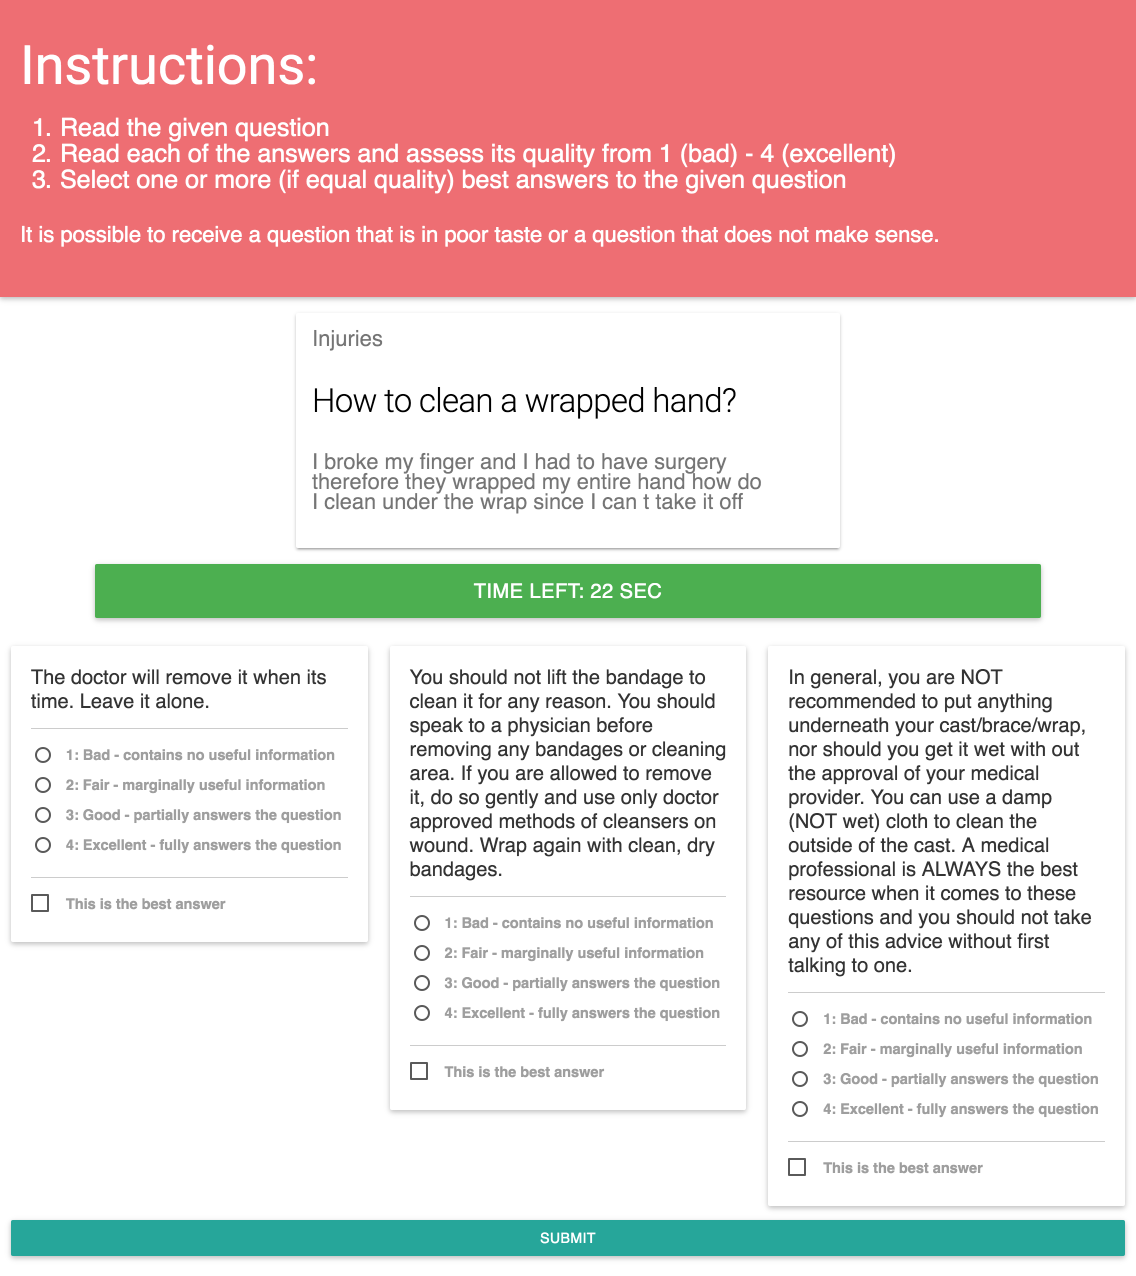
\includegraphics[width=1.0\textwidth]{img/validation_screenshot}
  \caption{Answer validation form}
  \label{fig:non-factoid:crowd:interfaces:validation}
  \end{subfigure}
  \begin{subfigure}[b]{0.45\textwidth}
  \centering
  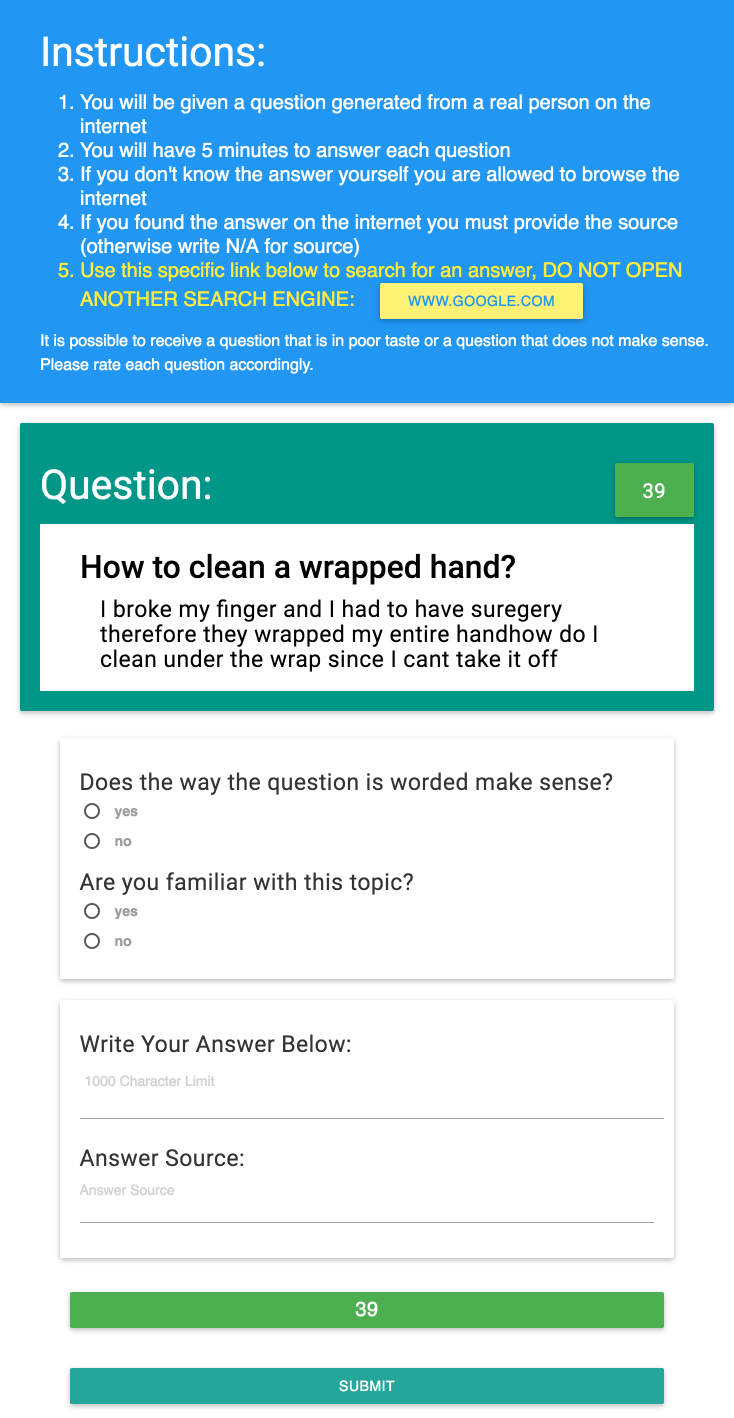
\includegraphics[width=0.9\textwidth]{img/answering_screenshot}
  \caption{Answer crowdsourcing form}
  \label{fig:non-factoid:crowd:interfaces:answer}
  \end{subfigure}
\caption{User interfaces for crowdsourcing answers and their judgements for TREC LiveQA questions}
\label{fig:non-factoid:crowd:interfaces}
\end{figure}

We chose to display 3 answers for a question, which were generated by three of the top-10 automatic systems from TREC LiveQA 2015 evaluation \cite{overviewliveqa15}.
To study the effect of time pressure on the quality of judgments we split participants into two groups. One group made their assessments with a 1 minute countdown timer shown to them, while the other could complete the task without worrying about a time limit.
Within each group, we assigned three different workers per question, and the workers were compensated at a rate of \$0.05 per question for this task.

The interface for collecting answer ratings is illustrated in Figure \ref{fig:non-factoid:crowd:interfaces:validation}\footnote{The screenshots show the final state of the form, as we describe later in this sections fields were unhidden step-by-step for proper timing of reading, answering and validation}.
On top of the interface workers were shown the instructions on the task, and question and answers were hidden at this time.
They were instructed to read the question, read the answers, and rate each answer's quality on a scale from 1 (Bad) to 4 (Excellent), and finally choose a subset of candidates that best answer the question.
Upon clicking a button to indicate that they were done reading the instructions, the question, a 60 second countdown timer and 3 answers to the question appeared on the screen.
At the 15 second mark the timer color changed from green to red.
In the experiments without time pressure the timer was hidden, but we still tracked the time it took for the workers to complete the task.

In this experiment we collected 6 ratings (3 with and 3 without time pressure) for each of three answers for a sample of 100 questions, which makes it a total of 1800 judgments.
Each answer also has an official NIST assessor rating on the same scale.
Figure \ref{figure:score_correlation} shows correlation between official NIST assessor relevance judgments and ratings provided by our workers.
The Pearson correlation between the scores is $\rho=0.52$.
The distribution of scores shows that official assessors were very strict and assigned many extreme scores of 1 or 4, whereas mechanical turk workers preferred intermediate 2s and 3s.
The results did not show any significant differences between experiments with and without time pressure.
Figure \ref{figure:validation_time} shows that even though the median time to rate all three answers is around 22-25 seconds in both experiments, the upper bound is significantly lower in the experiment with the time pressure.

\begin{figure}[t!]
	\centering
	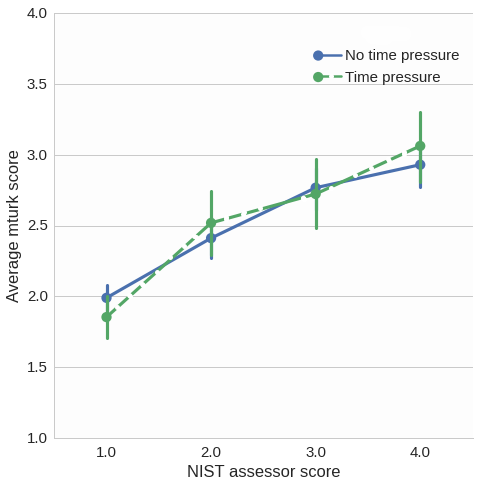
\includegraphics[width=0.35\textwidth]{img/score_correlation}
	\caption{Correlation between NIST assessor scores and crowdsourced ratings with and without time limit on the work time}
	\label{figure:score_correlation}
\end{figure}

\begin{figure}[t!]
	\centering
	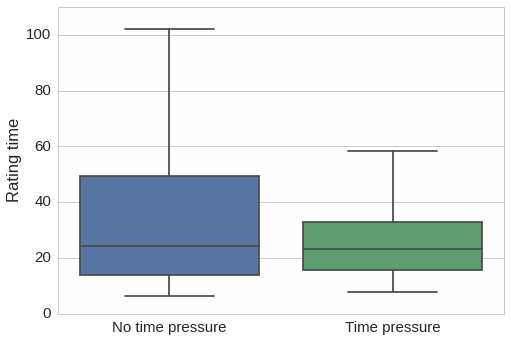
\includegraphics[width=0.4\textwidth]{img/validation_time}
	\caption{Box plot of answer rating time with and without time pressure}
	\label{figure:validation_time}
\end{figure}

Therefore, we conclude that in general we can trust crowdsourced ratings, and on average one minute is enough to judge the quality of three answers to CQA questions.

Next, we studied if crowd workers can provide an answer to a given question within a limited amount of time, we asked different workers to answer the questions from TREC LiveQA 2015.
We split the workers into two groups and displayed a one minute countdown timer for one of them.
We left a grace period and let the workers submit their answers after the timer had run out.
The workers received a \$0.10 compensation for each answer.
The form for answer crowdsourcing is shown in Figure \ref{fig:non-factoid:crowd:interfaces:answer}, and similar to the answer rating form, it starts with a set of instructions for the task.
We let the users browse the internet if they were not familiar with the topic or could not answer the question themselves.
To prevent them from finding the original question on Yahoo! Answers, we included a link to Google search engine with a date filter enabled\footnote{https://www.google.com/webhp?tbs=cdr:1,cd\_max:8/30/2015}.
Using this link, workers could search the web as it was on 8/30/2015, before TREC LiveQA 2015 questions were posted and therefore workers were in the same conditions as automatic systems on the day of challenge\footnote{The ranking of search results could be different on the day of the challenge and for our workers}.
Initially, the question was hidden for proper accounting of question-reading and answering times.
Upon clicking a button to indicate that they were done reading the instructions, a question appeared along with a button, which needed to be clicked to indicate that they were done reading the question.
After that, the answering form appears, it contained four fields:
\begin{enumerate}
\setlength{\itemsep}{0pt}
\setlength{\parskip}{0pt}
\item Does the question make sense: ``yes'' or ``no'' to see if the question was comprehensible
\item Are you familiar with the topic: A yes or no question to evaluate whether the worker has had prior knowledge regarding the question topic
\item Answer: the field to be used for the user's answer to the given question
\item Source: the source used to find the answer: URL of a webpage or NA if the worker used his own expertise
\end{enumerate}

We were able to collect 6 answers (3 with and without time pressure) for each of the 1087 LiveQA'15 questions.
Since we have answers from different sources, let's introduce the following notations:
\begin{itemize}
\setlength{\itemsep}{0pt}
\setlength{\parskip}{0pt}
	\item \textit{Yahoo! Answers} - answers eventually posted by users on Yahoo! Answers for the original questions
	\item \textit{Crowd} - answers collected from Mechanical Turk workers without time pressure
	\item \textit{Crowd-time} - answers collected from Mechanical Turk workers with one minute time pressure
	\item \textit{LiveQA winner} - answers from the TREC LiveQA'15 winning system
	\item \textit{LiveQA top10} - answers from another top 10 TREC LiveQA'15 system.
\end{itemize}

Table \ref{table:answer_stats} summarizes some statistics on the answers.
The first thing to notice is that, unlike CQA websites, where some questions are left unanswered, by paying the crowd workers we were able to get at least one answer for all LiveQA questions (after filtering ``No answer'' and ``I don't know'' kind of responses).
The length of the answers, provided by Mechanical turk users is lower, and time pressure forces users to be even more concise.
The majority of workers ($\sim90 \%$) didn't use the web search and provided answers based on their experience, opinions and common knowledge.

\begin{table*}[ht]
\centering
\caption{Statistics of different types of answers for Yahoo! Answers questions}
\begin{tabular}{| p{3cm} | c | c | c | c |}
\hline
Statistic & Y!A & mTurk & mTurk-time & LiveQA'15 winning system\\
\hline
\% answered & 78.7\% & 100.0\% & 100.0\% & 97.8\% \\
Length (chars) & 354.96 & 190.83 & 126.65 & 790.41 \\
Length (words) & 64.54 & 34.16 & 22.82 & 137.23 \\
\hline
\end{tabular}
\label{table:answer_stats}
\vspace{-0.3cm}
\end{table*}

From Figure \ref{fig:answering_time_distribution} we can see that adding time pressure shifts the distribution of answering times\footnote{We had separate timers for reading the instructions, the question, and writing the answer, the inclusion of instruction-reading time is why the total time could be more than 1 minute}.
The tail of longer work times for no time limit experiment becomes thin with time restrictions and the distribution peaks around one minute.

\begin{figure}[t!]
	\centering
	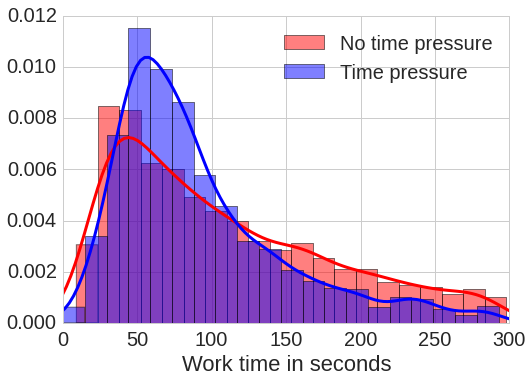
\includegraphics[width=0.4\textwidth]{img/answering_time_distribution}
	\caption{Distribution of answering times for experiments with and without time pressure}
	\label{fig:answering_time_distribution}
\end{figure}

Finally, to compare the quality of the collected answers with automatic system and CQA responses we pooled together the crowdsourced answers, the answers from the winning and other top-10 LiveQA'15 systems, and the original answers crawled from Yahoo! Answers for a sample of 100 questions.
Each answer was judged by 3 different workers (without time pressure), and their scores were averaged.
Figure \ref{fig:average_score} displays the plot with average score for answers from different sources.
Quite surprisingly the quality of collected answers turned out be comparable to those of CQA website users.
Average rating of answers produced by the winning TREC LiveQA system is also pretty close to human answers.
Finally, as expected, time pressure had its negative effect on the quality, however it is still significantly better than quality of an average top 10 QA system.

\begin{figure}[h]
	\centering
	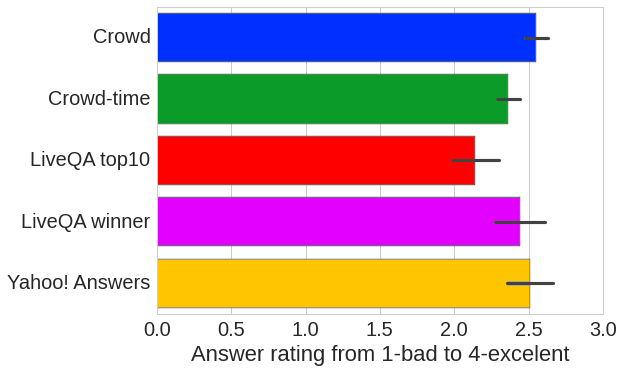
\includegraphics[width=0.4\textwidth]{img/average_score}
	\caption{Average scores of different types of answers to Yahoo! Answers questions}
	\label{fig:average_score}
\end{figure}

\begin{figure}[h]
	\centering
	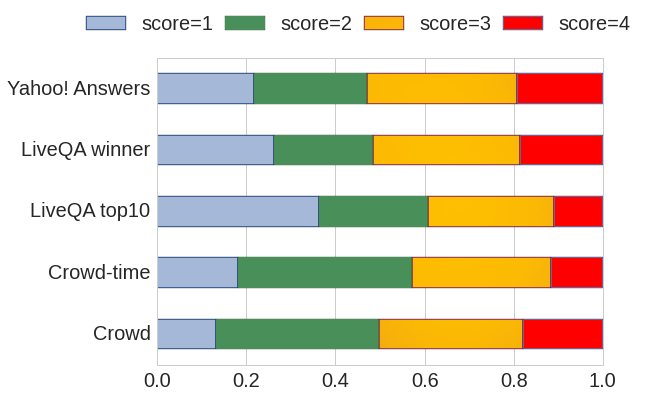
\includegraphics[width=0.4\textwidth]{img/scores_distribution}
	\caption{Distribution of scores for different types of answers to Yahoo! Answers questions}
	\label{fig:scores_distribution}
\end{figure}


Analysis of the score distribution (Figure \ref{fig:scores_distribution}) sheds some light on the nature of the problems with automatic and human answers.
The automated systems generate non-relevant answers ($score=1$) more often than human, either because the systems fail to retrieve relevant information, or to distinguish between useful and non-useful answer candidates.
However, by having a larger information store, e.g., the Web, automated QA systems can often find a perfect answer ($score=4$), while crowd workers tend to give generally useful, but less perfect responses ($score=2,3$).

Our initial results show that crowd workers are capable of validating a small set of answer candidates quickly, which could be potentially incorporated into an automatic QA system for answer validation and reranking.
In addition, even one minute appears enough for a crowd to generate a fair or good response to most real questions drawn from a CQA site, which can be useful in case a QA system didn't have good candidates in the first place.
The quality of crowdsourced answers was comparable to the original Yahoo! Answers responses, and even with time pressure, crowdsourcing was shown promising to complement or augment automated QA systems.
In the next section, I describe the proposed work on incorporating crowdsourcing into a real QA system.

\subsection{Integrating Crowdsourcing into a Real QA System}
\label{sec:non-factoid:crowd:integrating}

There are a number of questions, that need to be addressed in order to build an efficient real-time human-computer question answering system.
I'm planning to add crowdsourcing as a component to my TREC LiveQA 2016 system, which would require solving the problems of obtaining and retaining a set of workers for the duration of the challenge, designing a good user interface, developing a proper interaction model between an automated system and the workers, \etc.

The crowdsoucing module for our LiveQA system will represent a website, where workers from Amazon Mechanical Turk will enter and stay until we give them a task to do.
Here, we are building on the previous research on obtaining a crowd for real-time tasks, \eg \cite{bernstein2011crowds}.
The workers will be payed a small fixed rate for accepting the HIT and entering our QA interface and then by time they spent there responding and validating questions.
Inactive workers will be logged out of the system if they don't respond to an incoming question.
Figure \ref{fig:non-factoid:crowd:proposed:interface} shows the user interface of the crowdsourcing module of our TREC LiveQA system.
It displays the question and some potentially useful information for answering it (\eg search results).
A worker can type his own answer if he happen to know it, or she can judge the provided list of candidate answers.

\begin{figure}[t]
\centering

\includegraphics[width=0.9\textwidth]{img/nonfactoid_crowd_interface}
\caption{User interface for the crowdsourcing module of TREC LiveQA system}
\label{fig:non-factoid:crowd:proposed:interface}
\end{figure}

The interactions between the automated system and the crowdsourcing module will look the following way:
\begin{enumerate}
\item When a system receives a question, it is sent to the crowdsourcing UI, so workers could read it and possibly start responding if they happen to know the answer
\item Then a system generates a set of candidate answers, score them and send top candidates to the crowdsourcing module for validation
\item At the end of the alloted 1 minute period the crowdsourcing module responds back with the answer a worker possibly wrote as well as scores for validated candidate answers
\item The automated system aggregates this information and chooses whether to return the worker answer or to go with one of the existing candidates.
\end{enumerate}

%-=-=-=-=-=-=-=-=-=-=-=-=-=-=-=-=-=-=-=-=-=-=-=-=-=-=-=-=-=-=-=-=-=-=-=-
\section{Evaluation}
\label{sec:non-factoid:architecture:evaluation}

Evaluation of complete non-factoid question answering systems is complicated due to the variability of answer language, the quality of which is impossible to estimate using manually created answer patterns (as is the case for factoid TREC QA dataset).
A manual judgment of answers is needed, and luckily TREC LiveQA 2016 is offering such an opportunity.
The model I'm developing will participate in the shared task, which will allow us to evaluate it against other competing approaches.

The analysis of individual components can be performed using labeled data from TREC LiveQA 2015, which includes passages extracted from Yahoo! Answers as well as regular web documents.
In more detail, the performance of the answer summarization module will be estimated by similar questions retrieval performance, \eg Precision @ N since we are interested in retrieving more relevant answers in TopN rather than good ranking within the retrieved group.
To make results reproducible a collection of Yahoo! Answers QnA pairs from the WebScope\footnote{http://webscope.sandbox.yahoo.com/catalog.php?datatype=l} and Lucene IR library will be used for question retrieval.

The dataset to evaluate the effectiveness of using web page structure for answer scoring will be derived from TREC LiveQA 2015 labels, which include a big number of passages, that were generated from regular web pages.
Therefore, the problem of evaluation of answer scoring methods can be posed as passage ranking problem and metrics, such as Precision@1, can be used as a quality measure.

Finally, the answer summarization module is the most difficult to evaluate, because it's result is a free form text, the quality of which needs to be manually labeled.
Therefore, for this task I will refer to the wisdom of a crowd and use Amazon Mechanical Turk to label the quality of answers and compare to the top scoring passages for the same question.

\section{Summary}
\label{sec:non-factoid:summary}

The proposed research directions target various aspects of non-factoid question answering pipeline and can help improve both precision and recall of existing systems.
The results of this work can help to move in the direction of systems, that produce a natural language response by analyzing the information available on the web.
In the next chapter, I will describe the proposed work and results on interactions between a question answering system and users.

%THIS IS OLD...
%My proposal for non-factoid question answering can be summarized as follows:
%\begin{itemize}
%\setlength\itemsep{0em}
%\item \textbf{CQA candidate generation}: retrieve a set of question-answer pairs by searching a CQA archive\footnote{https://answers.yahoo.com/}
%\item \textbf{Web document retrieval}: retrieve a set of documents by querying web search with the question (and queries generated from it)
%\item \textbf{Web candidate answer generation}: classify web page into one of the following types: article, forum thread, FAQ page, CQA page, other. Extract key elements using type-specific extractors (QnA pairs, FAQ and CQA pages, forum question and posts and article passages with the corresponding titles, subtitles and surrounding text).
%\item \textbf{Ranking}: Rank the generated candidate answers by building on techniques from existing research \cite{surdeanu2011learning}.
%\end{itemize}
